% circles.m4
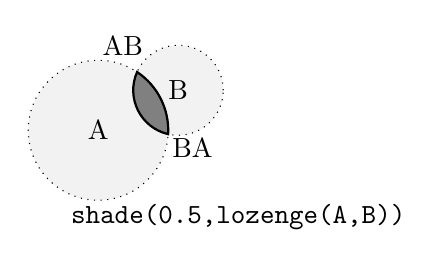
\begin{tikzpicture}[scale=2.54]
% dpic version 2020.09.01 option -g for TikZ and PGF 1.01
\ifx\dpiclw\undefined\newdimen\dpiclw\fi
\global\def\dpicdraw{\draw[line width=\dpiclw]}
\global\def\dpicstop{;}
\dpiclw=0.8bp
\dpicdraw[fill=white!95!black,line width=0.4bp,dotted](0.35,0) circle (0.137795in)\dpicstop
\draw (0.35,0) node{A};
\dpicdraw[fill=white!95!black,line width=0.4bp,dotted](0.75,0.2) circle (0.088583in)\dpicstop
\draw (0.75,0.2) node{B};
\draw (0.59428,0.351128) node[above left=-2bp]{AB};
\draw (0.69947,-0.019253) node[below right=-2bp]{BA};
\draw (1.05,-0.35) node[below=-2bp]{\tt shade(0.5,lozenge(A,B))};
\dpiclw=0.8bp
\global\let\dpicshdraw=\dpicdraw\global\def\dpicdraw{}
\global\def\dpicstop{--}
\dpicshdraw[fill=white!50!black]
\dpicdraw (0.54428,0.291128)
 ..controls (0.48703,0.161889) and (0.561729,0.012491)
 ..(0.69947,-0.019253)\dpicstop
\dpicdraw (0.69947,-0.019253)
 ..controls (0.706281,0.104374) and (0.647268,0.2224)
 ..(0.54428,0.291128)\dpicstop
cycle; \global\let\dpicdraw=\dpicshdraw\global\def\dpicstop{;}
\end{tikzpicture}
